\section{PR2 Introduction}
\begin{frame}
  \frametitle{Introduction}
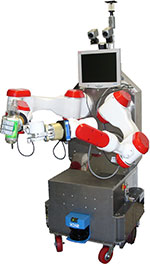
\includegraphics[width=2cm]{img/taser.jpg}
\hspace{5ex}
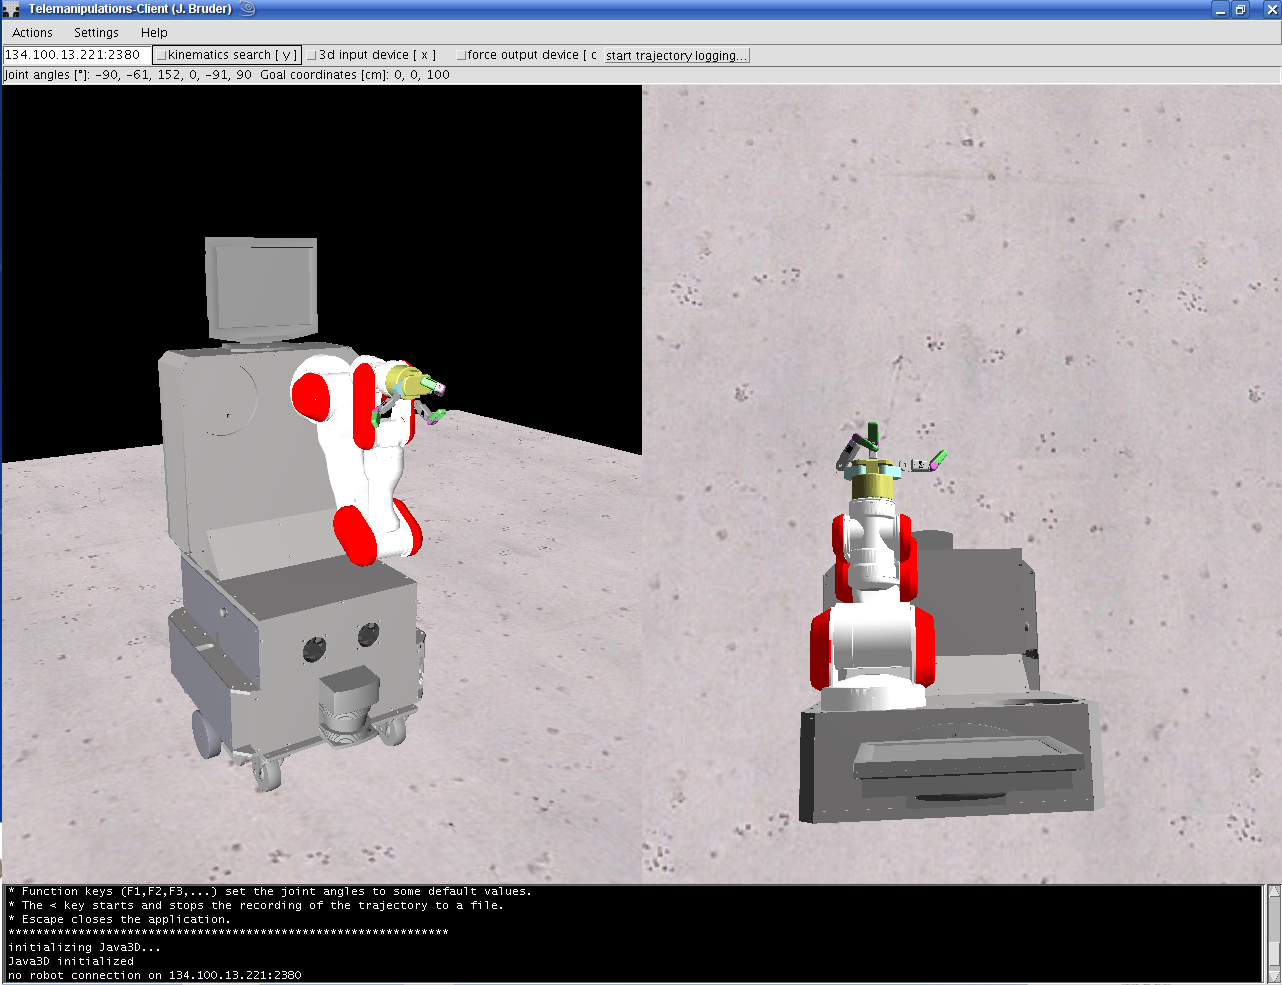
\includegraphics[width=5cm]{img/TASER_simulator1.png} \\[0cm]
\vspace{-6ex}
\hspace{33ex}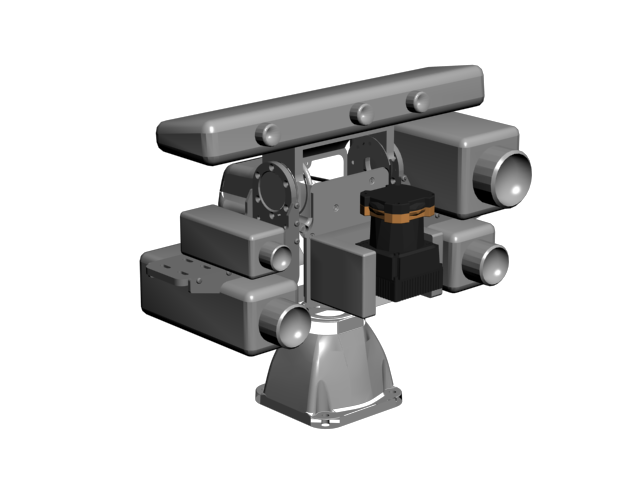
\includegraphics[width=5cm]{img/ActivePerceptionStereoHead_Top_Front.png}
\end{frame}


\section{PR2 Overview}
\begin{frame}
  \frametitle{PR2}
\hspace{-3ex}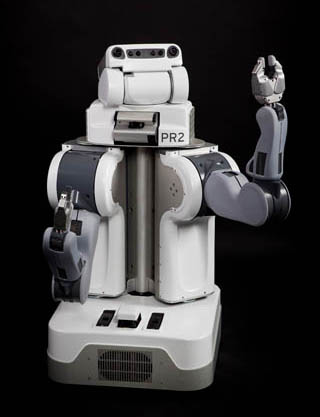
\includegraphics[width=3cm]{img/PR2_front.jpeg} 
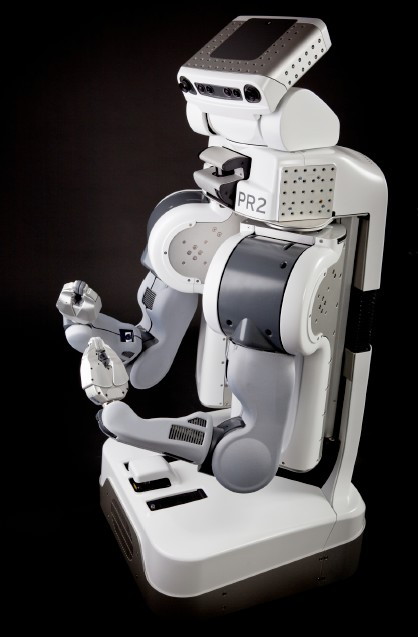
\includegraphics[width=2.57cm]{img/PR2_side.jpeg} 
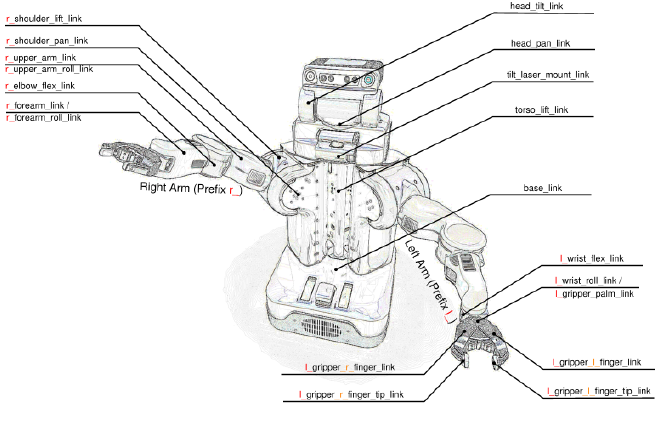
\includegraphics[width=6cm]{img/pr2_link_name.png}
\end{frame}

\begin{frame}
  \frametitle{PR2 - Users}
\centering\includegraphics[width=12cm]{img/pr2_users.pdf} 
\end{frame}

\begin{frame}
  \frametitle{PR2 - Hardware Specification}
\begin{itemize}
    \item $2\times$ computers with 24 Gb RAM and quad-core Nehalem processors
    \item 1.3 kWh Lion Battery Pack
    \item 2 hrs Approximate Runtime
    \item Coordinate system (for all links) positive z-axis up, positive x-axis forward, and positive y-axis robot-left when PR2 in the home pose
    
\end{itemize}
\end{frame}


\begin{frame}
  \frametitle{The PR2 motion control layout}
\hspace{15ex}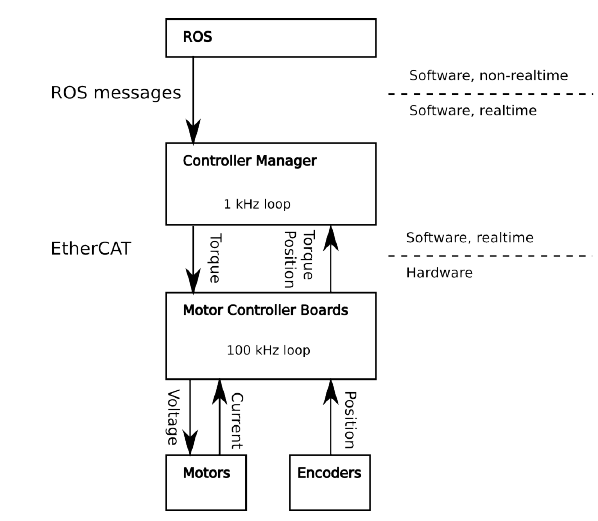
\includegraphics[width=7cm]{img/motion_control.png} 
\end{frame}

\begin{frame}
  \frametitle{Network explanation}
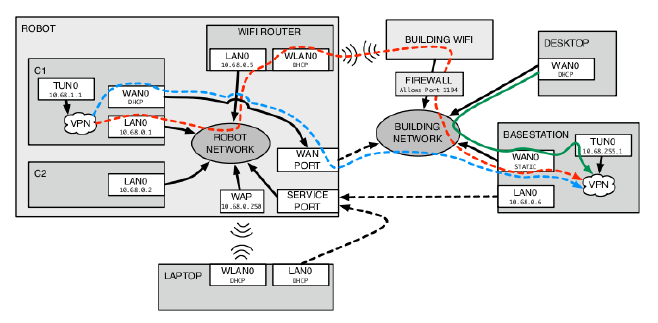
\includegraphics[width=12cm]{img/network.png} 
\end{frame}


\begin{frame}
  \frametitle{PR2 - Hardware Specification}
\small{
\begin{itemize}
    \item Arm DOFs: arm 4 (A), wrist 3 (B), gripper 1 (C)
    \item Link Lengths: upper arm 400\,mm, forearm 321\,mm,\\ wrist to gripper surface 120 - 200\,mm
    \item Range of motion: shoulder pan/tilt $170^0/115^0$,\\ upper arm roll $270^0$, elbow flex $140^0$, forearm \\roll continuous, wrist pitch/roll $130^0$/continuous, \\gripper 90\,mm max
    \item Force output: 4 DOF passive counterbalance, \\arm payload 1.8\,Kg, wrist torque 4\,Nm, \\grip force 80\,N
    
\end{itemize}
}
\vspace{-13ex}\hspace{47ex}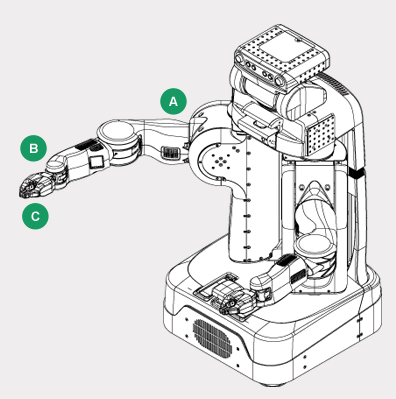
\includegraphics[width=3.4cm]{img/pr2_arm.png} 
\end{frame}

\begin{frame}
  \frametitle{PR2 - Intrinsic sensors}
\begin{itemize}
    \item Microstrain 3DM-GX2 IMU (above the shoulders)
    \item Three-Axis Accelerometer (gripper)
    \item Calibration LED (gripper) 
\end{itemize}
\end{frame}

\begin{frame}
  \frametitle{PR2 - Extrinsic sensors - Head}
\begin{itemize}
    \item Microsoft Kinect (color/depth image/point cloud $[640\times480 @ 30\,fps]$)
    \item Global shutter color gigabit ethernet camera (Prosilica GC2450C, 5\,MP, $[2448\times2050 @ 15\,fps]$)
    \item Wide stereo camera system (Aptina MT9V032C12STC, 100\,Mb color ethernet, $[752\times480@15\,fps]$)
    \item Narrow stereo system (Aptina MT9V032C12STM, 100\,Mb monochrome ethernet, $[752\times480@15\,fps]$)    
    \item LED textured light projector (triggered with narrow-angle stereo camera)
\end{itemize}
\end{frame}

\begin{frame}
  \frametitle{PR2 - Extrinsic sensors - II}
\begin{itemize}
    \item Tilting laserscanner (Hokuyo UTM-30LX, $135^0 (+90^0 to -45^0)$,above the shoulders)
    \item Laserscanner (Hokuyo UTM-30LX, base)
    \item Global shutter gigabit ethernet camera ($2\times$, forearm)
    \item Fingertip pressure sensor arrays (gripper)
    \item Speaker
\end{itemize}
\hspace{-4ex}
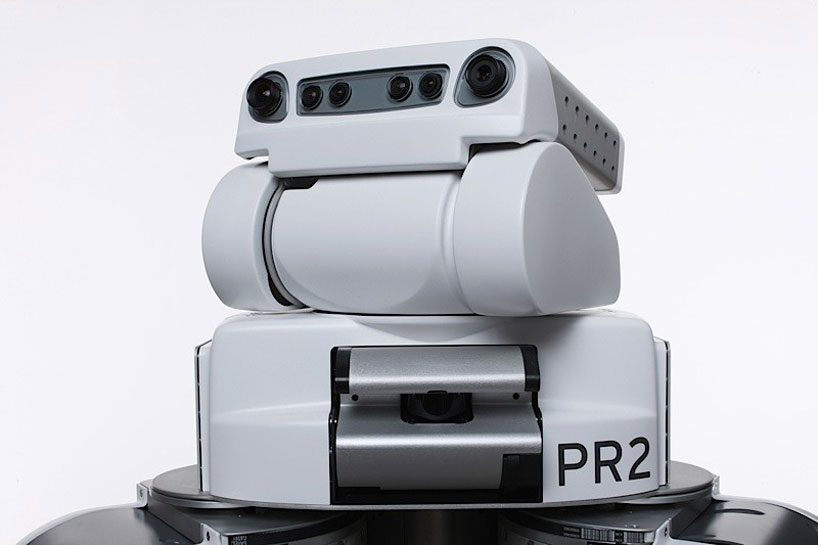
\includegraphics[width=4cm]{img/head_tiltLRF.jpg} 
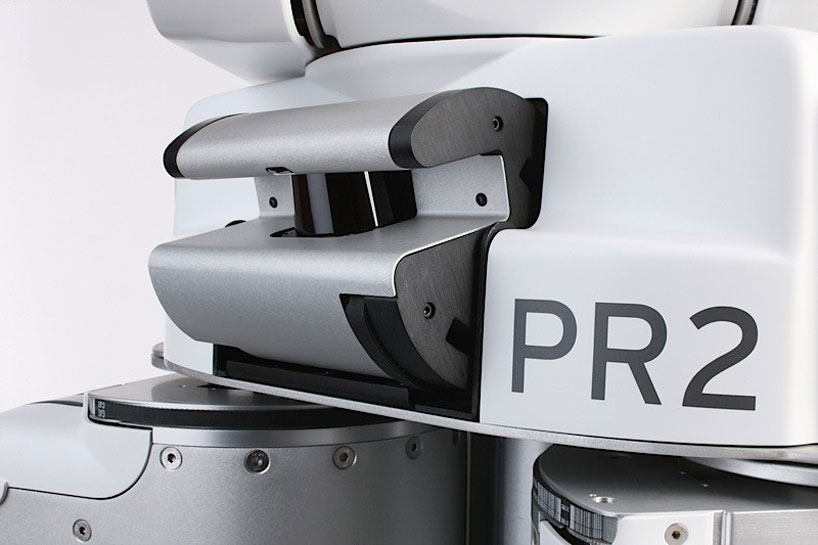
\includegraphics[width=4cm]{img/tilted_lrf.jpg}
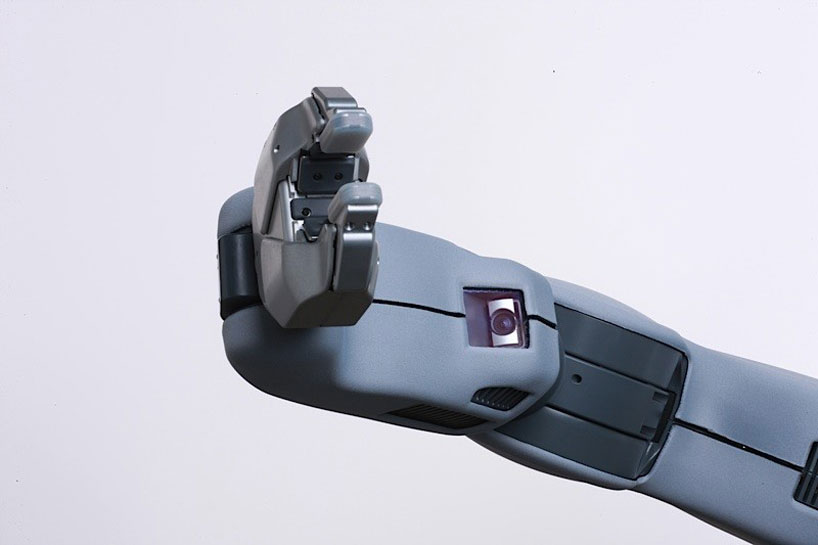
\includegraphics[width=4cm]{img/pr2_hand_camera.jpg}  
\end{frame}
